\section{Geometry and Functions}

\subsection{Equations of lines and circles}
\label{subsec:lines}

\begin{learningoutcomes} 
    \item Define geometric properties of straight lines and circles algebraically.
    \item Solve geometric problems involving lines and circles.
\end{learningoutcomes}

\subsubsection{Equation of a straight line}

An equation of the form
\[
ax+by=p
\]
for variables $x$ and $y$, and constants $a$, $b$ and $p$, represents a straight line in $x$--$y$ space. The equation can be rearranged into other forms. The form $y=mx+c$ is particularly useful. Here, $m$ represents the \textbf{gradient} of the line and $c$ represents the $y$-\textbf{intercept}, \textit{i.e.} the point $(0,c)$ where the line meets the $y$-axis (figure \ref{fig:line}). 
\begin{figure}[h!]
    \centering
    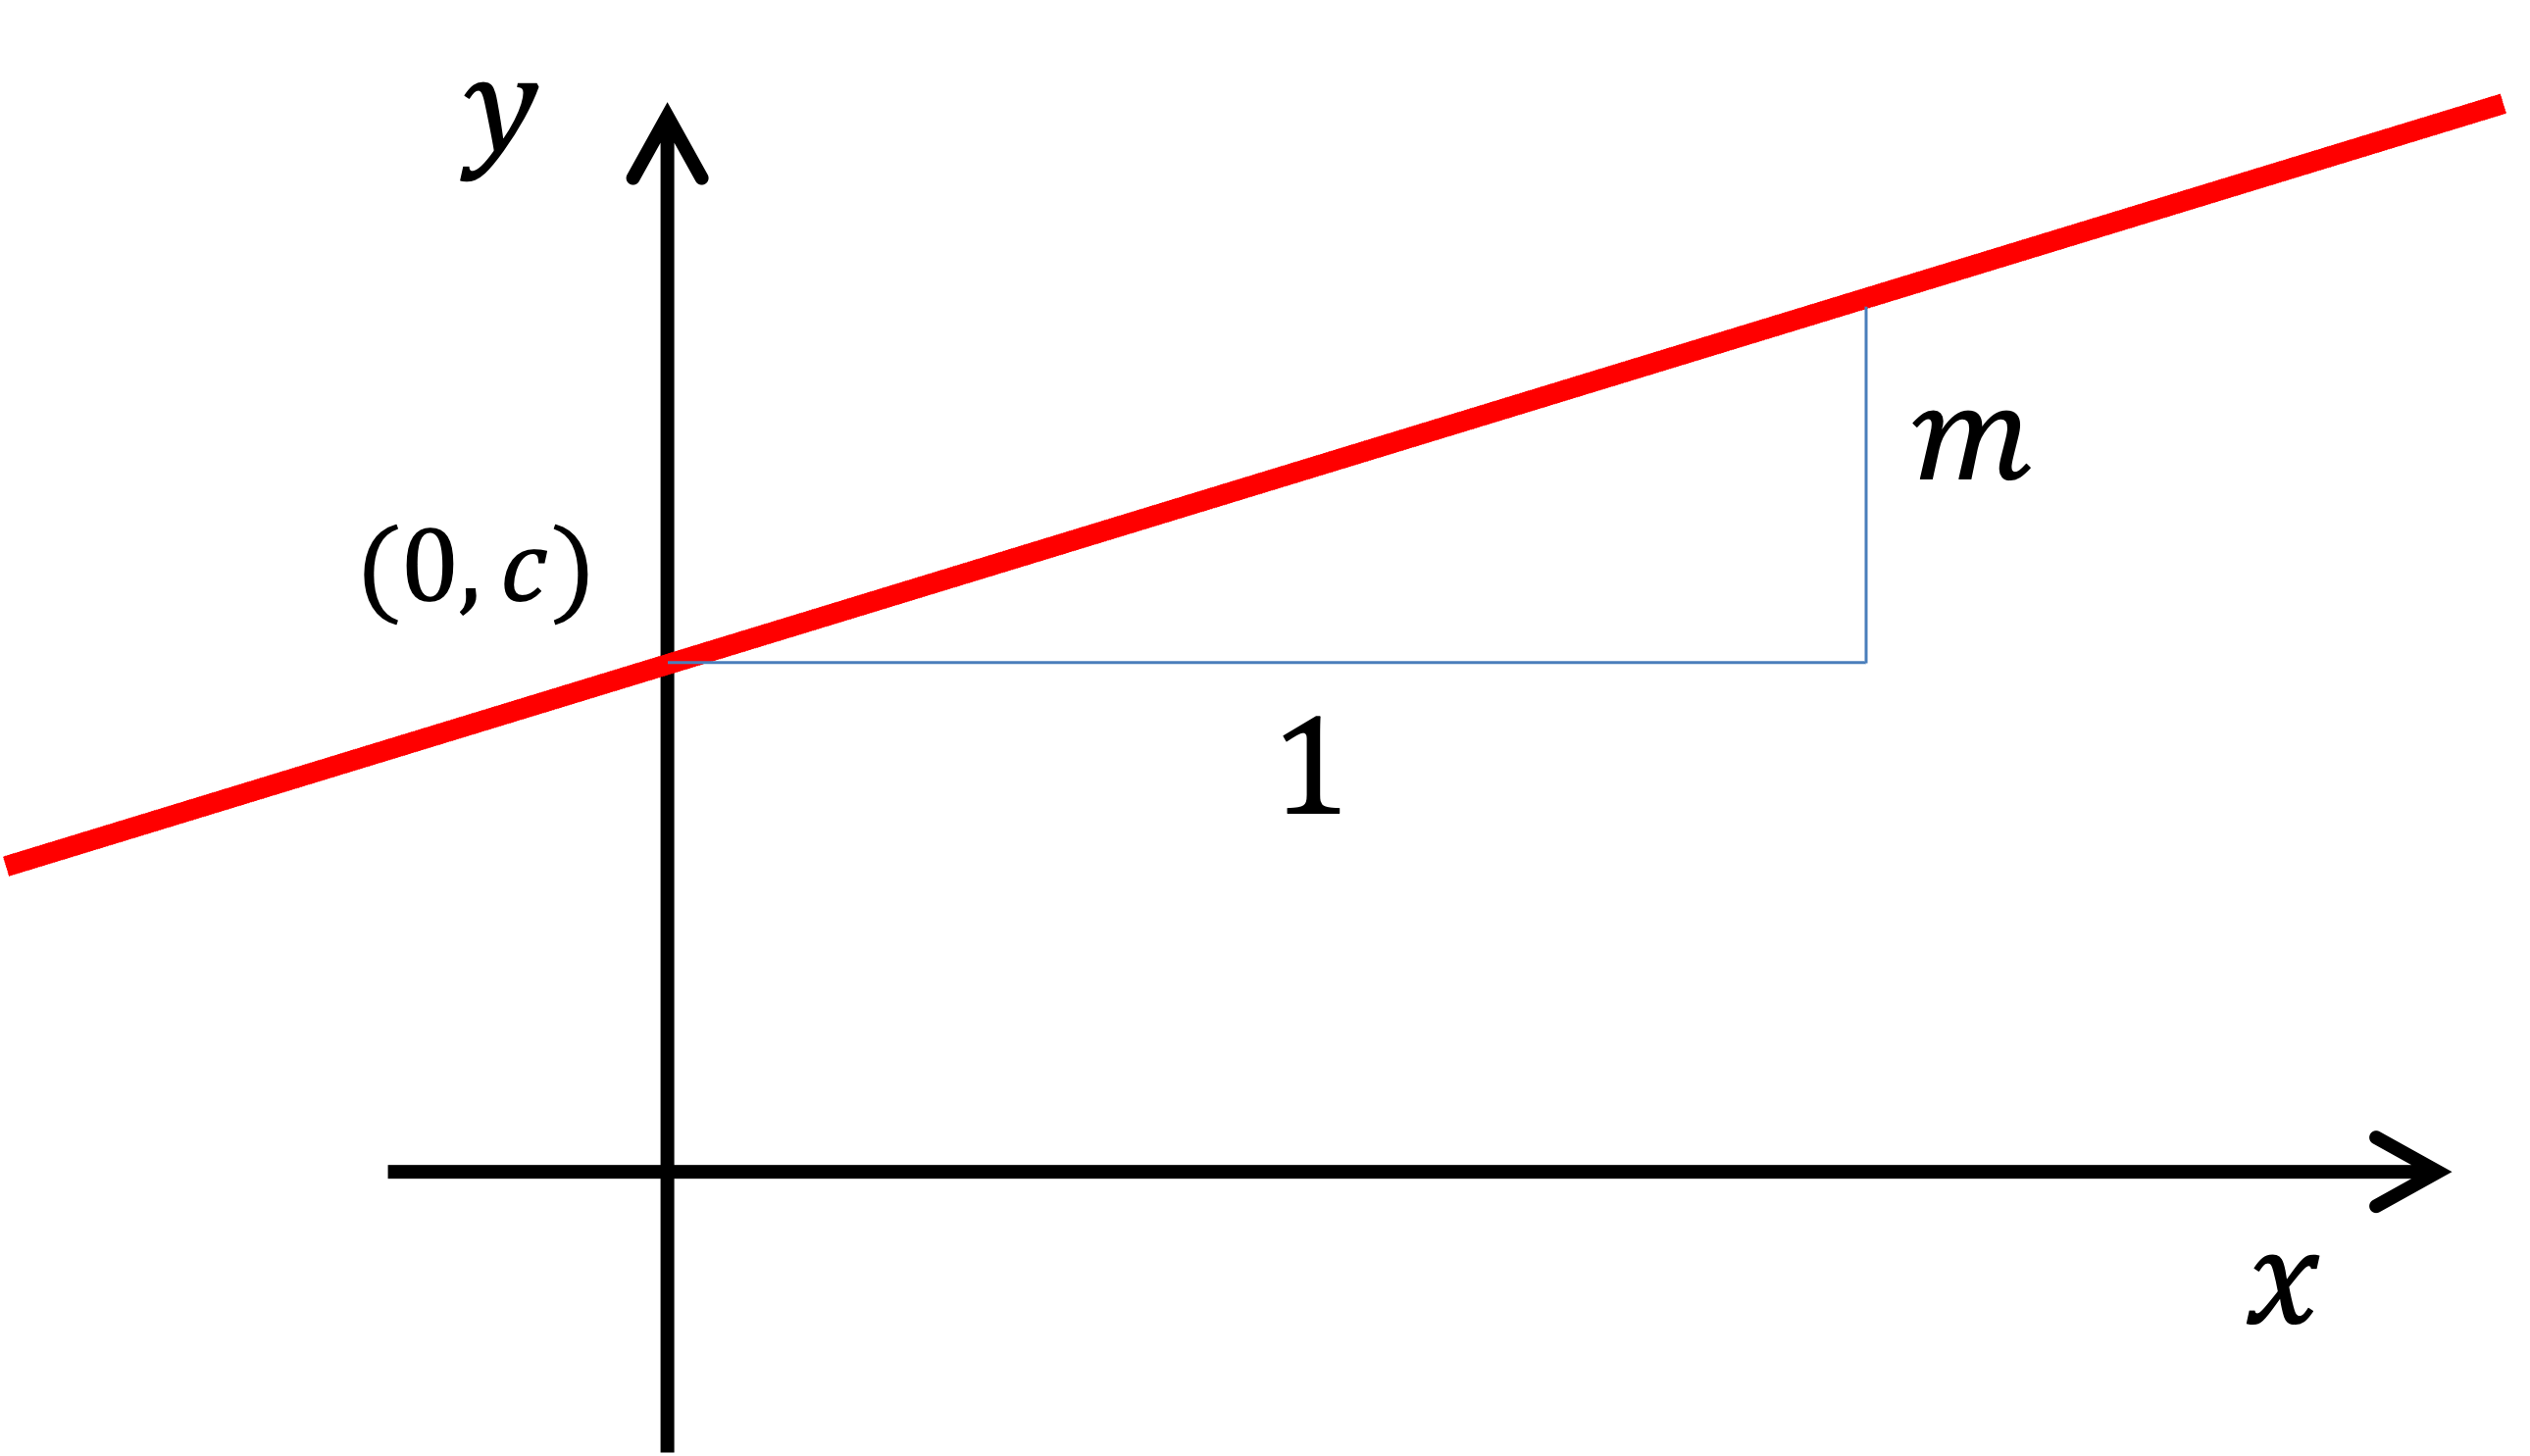
\includegraphics[width=0.5\textwidth, alt={Sketch of $y=mx+c$, showing that the y-coordinate of the line increases by $m$ for every distance 1 moved in the x-direction.}]{Figures/Section1/111a_line.png}
    \caption{Sketch of $y=mx+c$, showing that the y-coordinate of the line increases by $m$ for every distance 1 moved in the x-direction.}
    \label{fig:line}
\end{figure}
The animation in figure \ref{anim:straightline} (online version only) allows you to control the gradient and intercept of a straight line with sliders. 

\begin{figure}
    \iflatexml
        \<script src="https://cdn.jsdelivr.net/npm/chart.js">\</script>
        \<div class="chart-container">
        \<canvas id="lineChart" width="500" height="500">\</canvas>
        \</div>
        \<div class="slider-container">
        \<label class="slider-label" for="slopeSlider">Slope (m):\</label>
        \<input type="range" id="slopeSlider" min="-2" max="2" step="0.1" value="1"/>
        \<span id="slopeValue" class="slider-value">1\</span>
        \</div>
        \<div class="slider-container">
        \<label class="slider-label" for="interceptSlider">Intercept (c):\</label>
        \<input type="range" id="interceptSlider" min="-5" max="5" step="0.2" value="0"/>
        \<span id="interceptValue" class="slider-value">0\</span>
        \</div>
        \<script src="bmluser/straight\_line\_widget.js">\</script>
        \caption{Interactive plot of a straight line.}
    \else
        \centering
        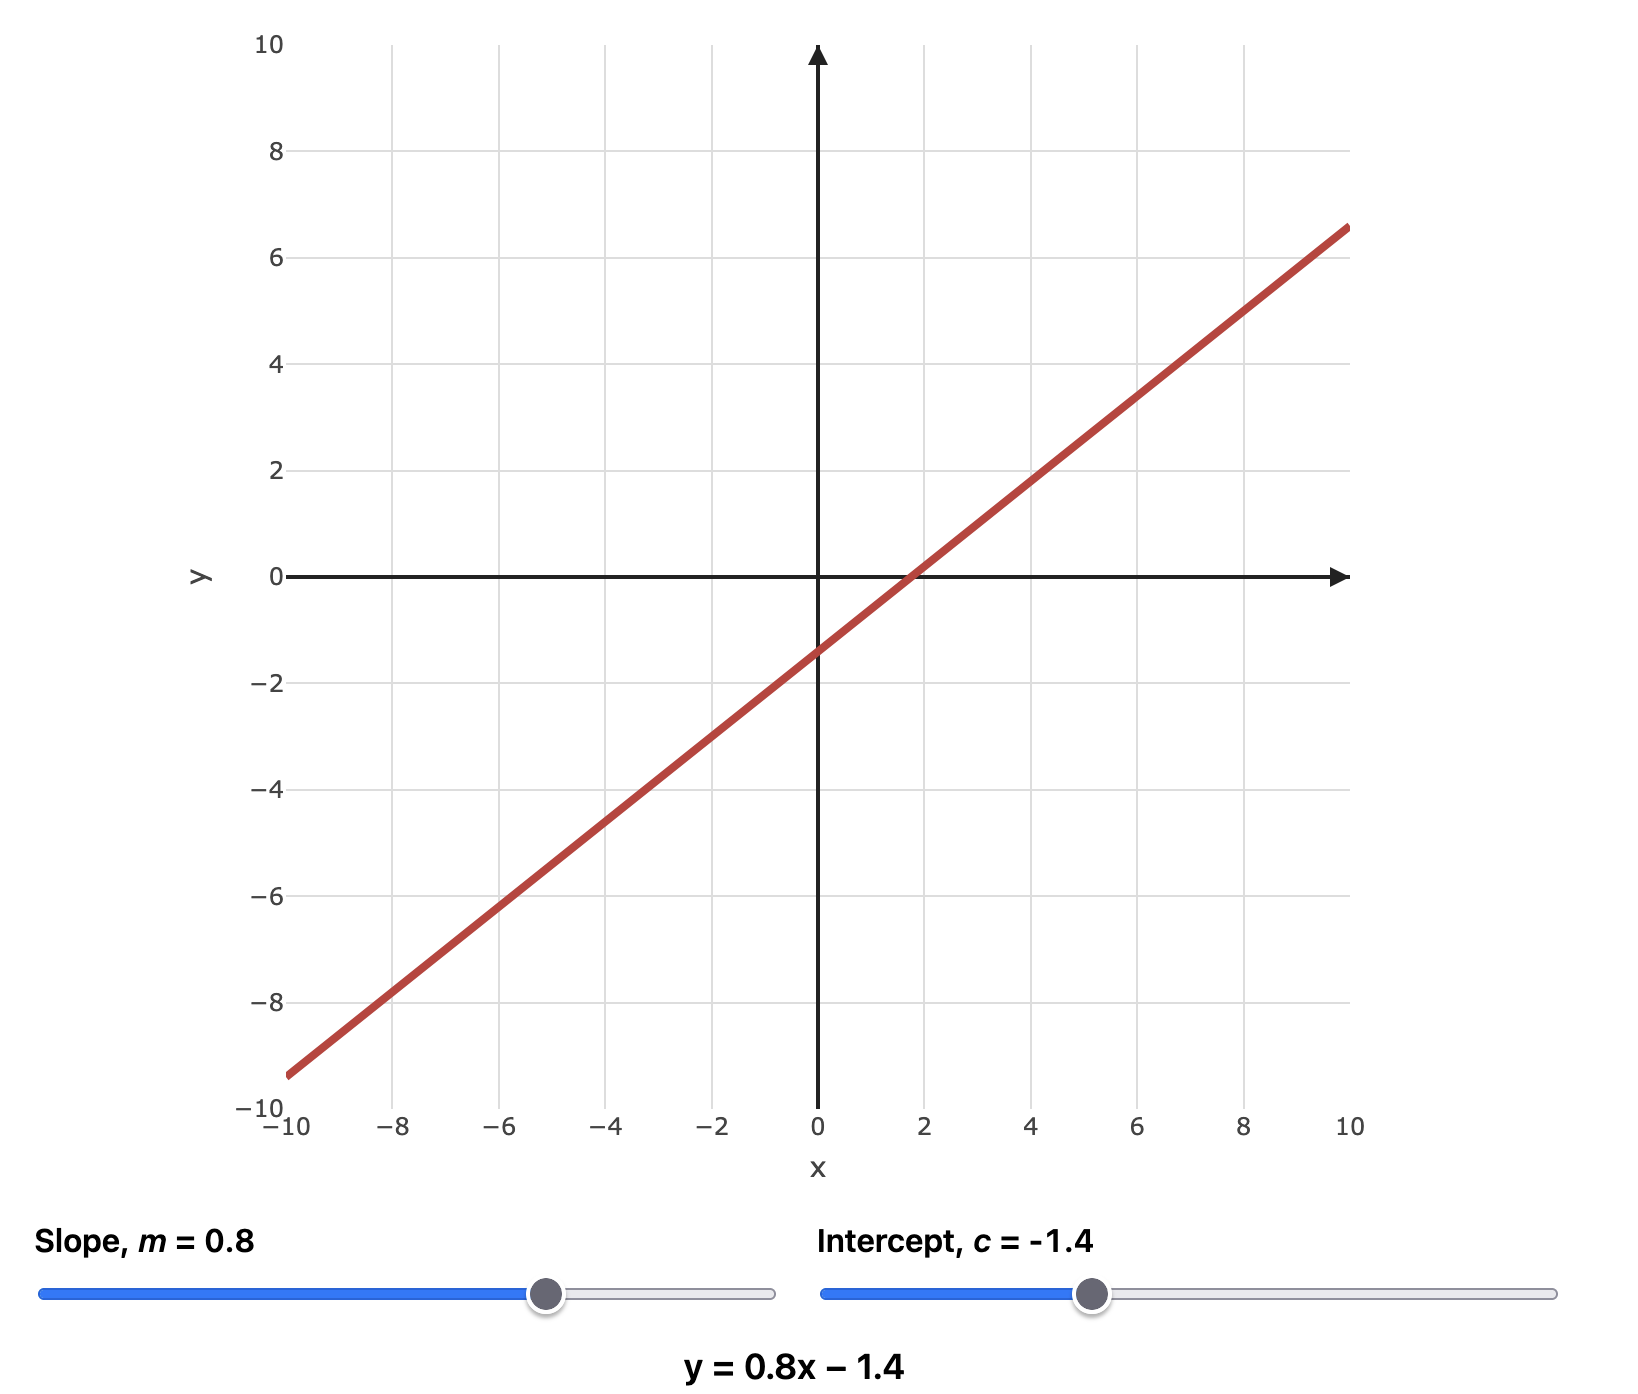
\includegraphics[width=0.5\textwidth]{Figures/Section1/straight_line_widget.png}
        \caption{Screenshot of the interactive plot of a straight line, available in the html version of these notes.}
    \fi
    \label{anim:straightline}
\end{figure}



Some useful properties of straight lines, as demonstrated in figure \ref{fig:lines_props}, are as follows
\begin{enumerate}[(a)]
    \item Two lines are parallel if they have the same gradient. For example, $y=x/2+3$ and $y=x/2$ are parallel. 
    \item Two lines are perpendicular if the product of their gradients is $-1$. For example, $y=-3x+5$ and $y=x/3$ are perpendicular.
    \item  A horizontal line has equation $y=c$.
    \item A vertical line has equation $x=d$. 
    \item Two lines cross at a point where they have the same value of $y$ for a given value of $x$.
\end{enumerate}

\begin{figure}[h!]
\centering
\subfig{0.45}{Figures/Section1/111bi_parallel.png}{Parallel lines}
\hfill
\subfig{0.45}{Figures/Section1/111bii_perp.png}{Perpendicular lines}
\hfill
\subfig{0.45}{Figures/Section1/111biii_horizontal.png}{Horizontal line}
\hfill
\subfig{0.45}{Figures/Section1/111biv_vertical.png}{Vertical line}
\hfill
\subfig{0.45}{Figures/Section1/111bv_crossing.png}{Two lines that cross}
\caption{Examples of straight line properties and relations.}
\label{fig:lines_props}
\end{figure}
 
\newtexpage
\begin{example}[DIY]
Find the crossing point of the lines
\[
y=-\frac{1}{2}x+4, \qquad y=x+1.
\]
\end{example}

\begin{blanksol}
Equate the two expressions for $y$:
\[
-\frac{1}{2}x+4=x+1.
\]
Rearranging gives $3=3x/2$, and hence $x=2$. Substitution into the second equation gives $y=2+1=3$. Therefore,
\[
(x,y)=(2,3).
\]
\end{blanksol}

\newtexpage
\subsubsection{Equation of a circle}

The equation of a circle with centre $(a,b)$ and radius $R$ is
\[
(x-a)^2+(y-b)^2=R^2 \,.
\]
The straight-line distance between two points $(x_1,y_1)$ and $(x_2,y_2)$ is
\[
d=\sqrt{(x_2-x_1)^2+(y_2-y_1)^2} \,.
\]
Thus, the radius $R$ is the distance from any point $(x,y)$ on the circle to its centre, which makes sense! (See figure \ref{fig:circle}).
\[
R=\sqrt{(x-a)^2+(y-b)^2}.
\]

\begin{figure}[h!]
    \centering
    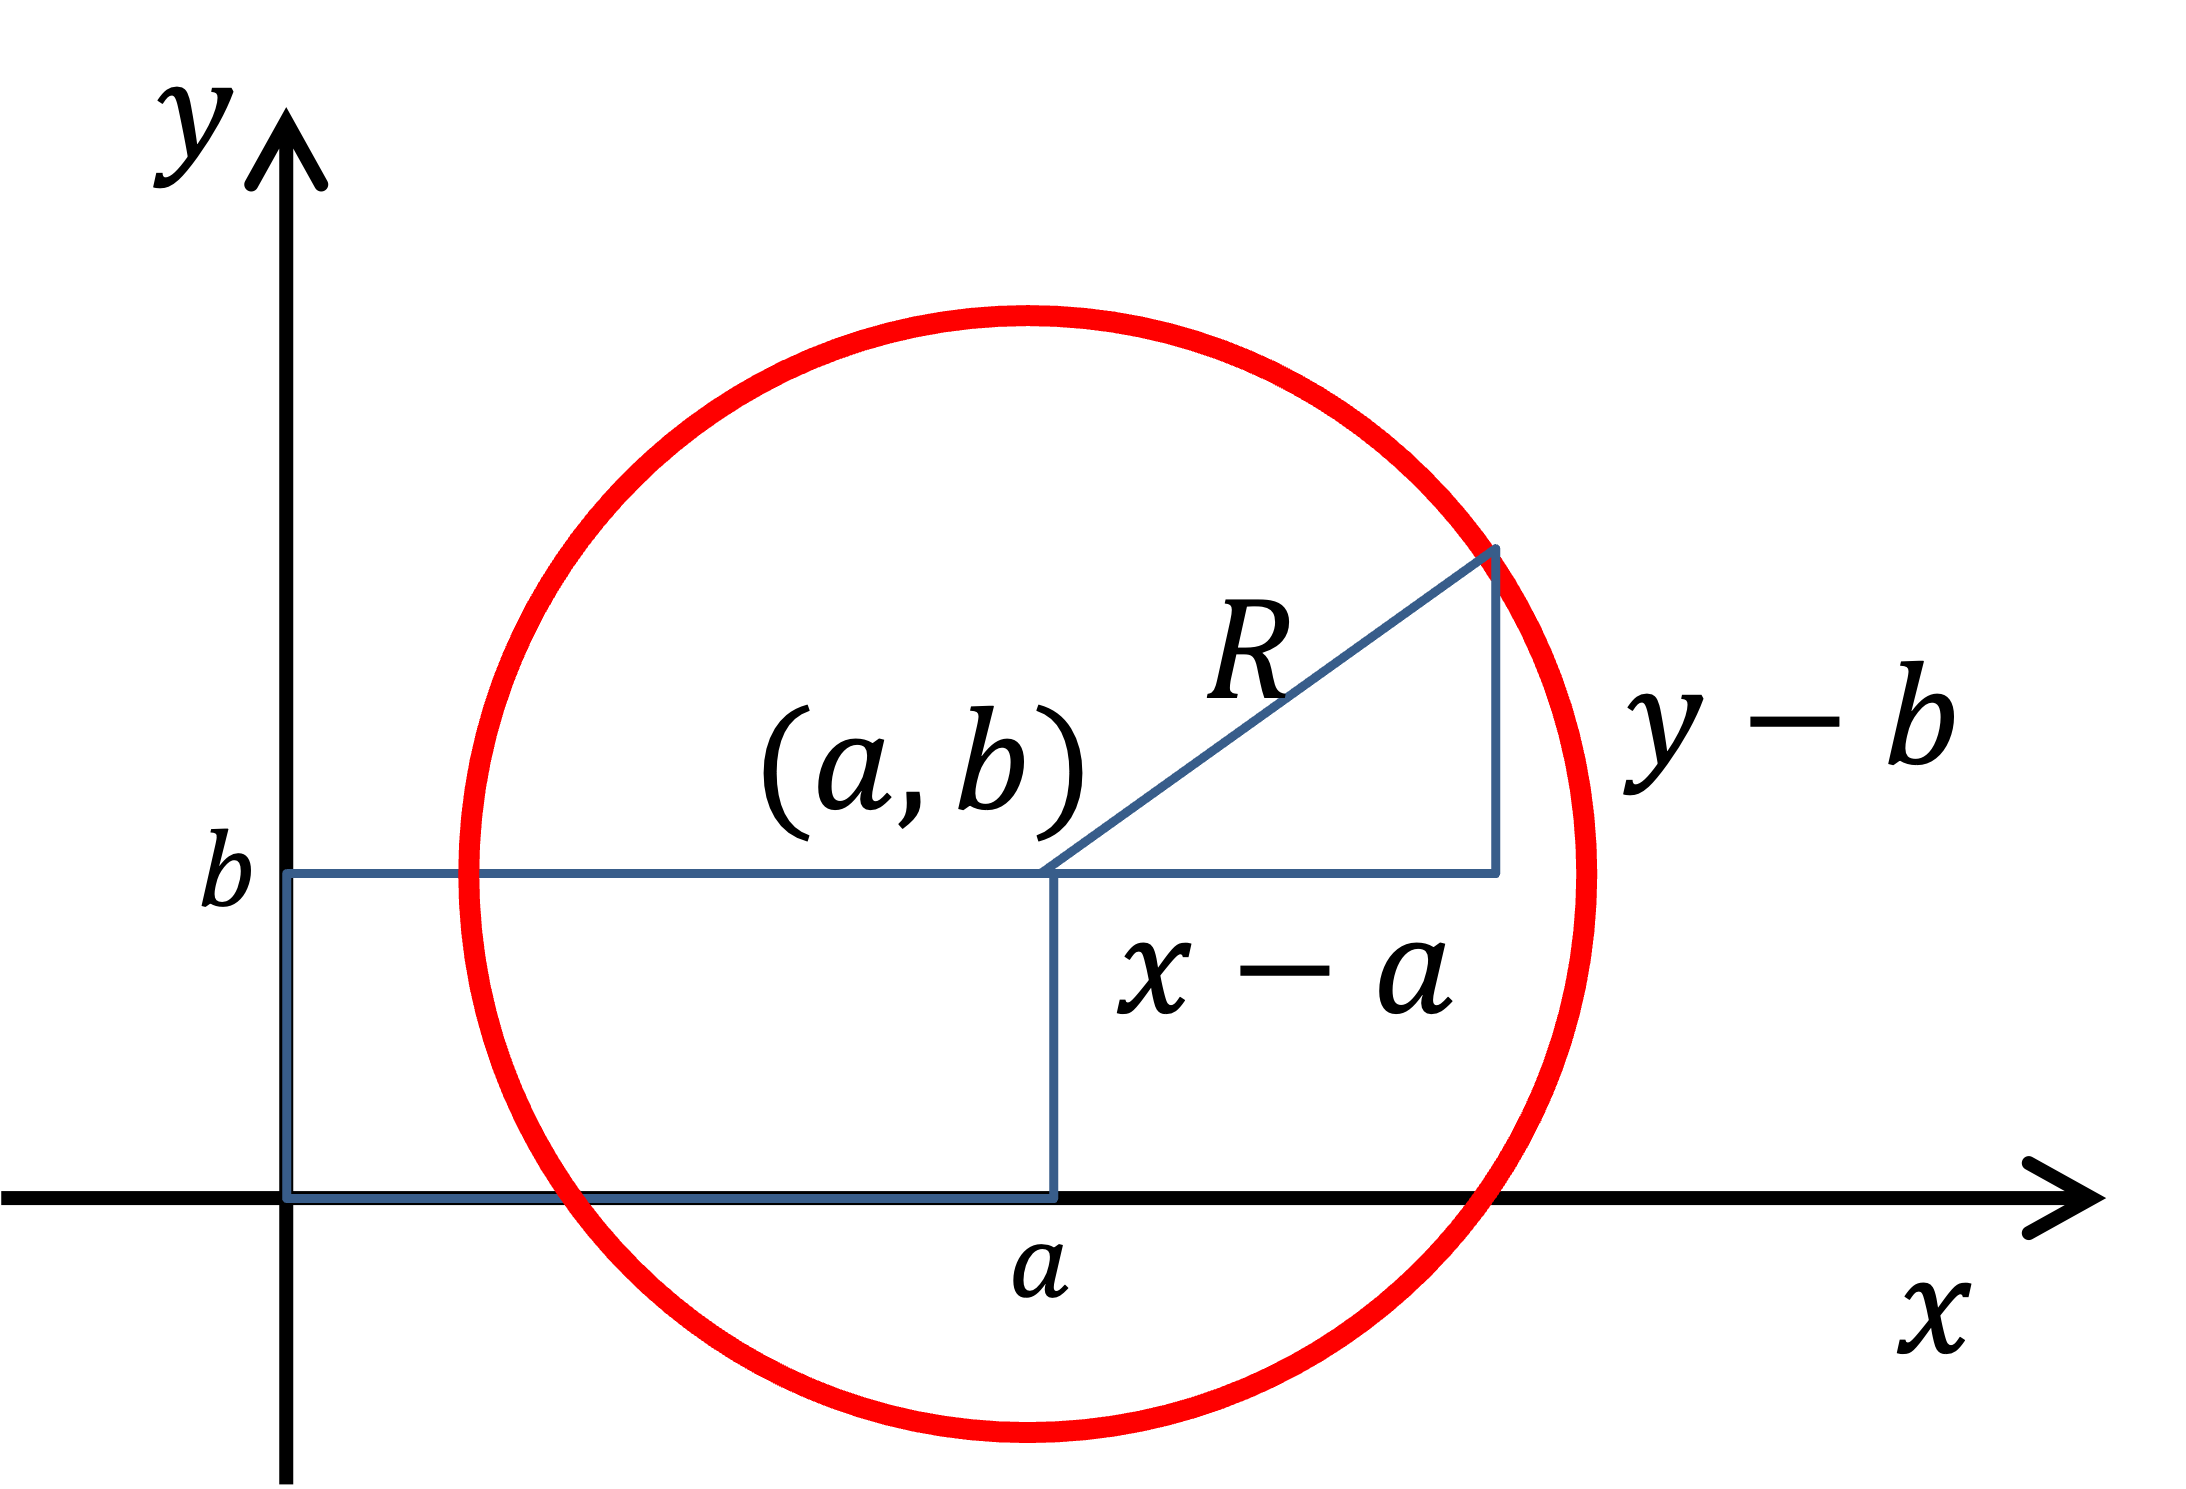
\includegraphics[width=0.5\linewidth]{Figures/Section1/112a_circle.png}
    \caption{Sketch of a circle, with centre ($a$,$b$) and radius $R$, which is also the hypotenuse of the right-angled triangle with side lengths $x-a$ and $y-b$.}
    \label{fig:circle}
\end{figure}

\begin{example}[Video]
Find the centre and radius of the circle with equation
\[
x^2+4x+y^2-6y=3.
\]
\end{example}

\begin{solution}
Complete the square for the quadratics in $x$ and $y$:
\[
\blank{x^2+4x=(x+2)^2-4}\, , \qquad \blank{y^2-6y=(y-3)^2-9}.
\]
Substitute these expressions back into the equation for the circle:
\[
\blank{(x+2)^2-4+(y-3)^2-9=3} \,, 
\]
so
\[
\blank{(x+2)^2+(y-3)^2=16} \,.
\]
Recall that the equation of a circle with centre $(a,b)$ and radius $R$ is $(x-a)^2+(y-b)^2=R^2$. Therefore,
\[
a=\blank{-2}\,, \qquad b=\blank{3}, \qquad R=\blank{4}.
\]
\end{solution}

To find where a line and a circle cross, substitute the equation of the line, $y=mx+c$, into the equation of the circle, $(x-a)^2+(y-b)^2=R^2$. This gives a quadratic equation for $x$, which may yield
\begin{itemize}
    \item two solutions: the line and circle cross twice.
    \item one repeated solution: the line is tangent to the circle
    \item no solutions: line and circle do not cross.
\end{itemize}
These possibilities are shown in figure \ref{fig:circle_cross}.
\begin{figure}[h!]
\centering
\subfig{0.3}{Figures/Section1/112_twocross.png}{Two crossing points}
\hfill
\subfig{0.3}{Figures/Section1/112_onecross.png}{One crossing point}
\hfill
\subfig{0.3}{Figures/Section1/112_nocross.png}{No crossing points}
\caption{Three possibilities for the crossing points of a line and a circle.}
\label{fig:circle_cross}
\end{figure}

\begin{example}[Lecture]
Do the following line and circle cross? If so, at what point or points?
\[
y=x+1, \qquad (x-1)^2+(y-2)^2=8.
\]
\end{example}

\begin{solution}
Substitute the line equation into the circle and rearrange, 
\begin{align*}
    \blank{(x-1)^2 + (x+1-2)^2} &= \blank{8} \\
    \blank{\therefore 2(x-1)^2} &= \blank{8} \, .
\end{align*}
Solve the resulting quadratic
\begin{align*}
    \blank{x-1} &= \blank{\pm 2}\\
    \therefore x &= \{\blank{-1},\; \blank{3}\} \, .
\end{align*}
then substitute the solutions into the line equation to get
\[
    y = \{\blank{0},\blank{4}\} \, ,
\]
respectively. \par
Therefore, the line and circle cross at $(\blank{-1},\blank{0})$ and $(\blank{3},\blank{4})$.
\end{solution}

At any point on a circle, the radius and tangent are perpendicular, as shown in figure \ref{fig:perp_rad}(a). 

\begin{definition}
    The \textbf{perpendicular bisector} of a line segment $AB$ is a straight line that passes through the midpoint of $AB$ and is perpendicular to it.
    A straight line segment connecting two points on a circle is a \textbf{chord}.
\end{definition}

\textbf{Perpendicular bisector theorem:} Given two points $A$ and $B$, all points of the perpendicular bisector of the line segment $AB$ will be the same distance from $A$ and $B$. Therefore, if $A$ and $B$ lie on a circle, the perpendicular bisector of the chord $AB$ will pass through the centre, as shown in figure \ref{fig:perp_rad}(b). 

\begin{figure}[h!]
    \centering
    \subfig{0.45}{Figures/Section1/112bi_radtan.png}{Tangent line}
    \hfill
    \subfig{0.45}{Figures/Section1/112biI_perpbisector.png}{Perpendicular bisector}
    \caption{Sketches of (a) the tangent to a circle, which is perpendicular to its radius and (b) the perpendicular bisector ($CD$) of two points on the circle ($A$ and $B$), which passes through the circle's centre $E$.}
    \label{fig:perp_rad}
\end{figure}

\newtexpage
\begin{example}[Lecture]
Find the equation of a circle with centre along the line $y=2x-3$ and which also passes through $(1,6)$ and $(5,2)$.
\end{example}

\begin{solution}
Use the perpendicular bisector theorem. The gradient between the points is
\[
\frac{\Delta y}{\Delta x}=\blank{-1} \,.
\]
The midpoint is
\[
\left(\frac{x_1+x_2}{2},\frac{y_1+y_2}{2}\right)=\blank{(3,4)}\, .
\]
Therefore, the equation of the perpendicular bisector is
\[
\blank{y=x+1}\, .
\]
The centre is the crossing point of the perpendicular bisector with $y=2x-3$:
\[
\blank{(a,b)=(4,5)}\,.
\]
To find $R$, substitute any point on the circle:
\[
\blank{R^2=(1-4)^2+(6-5)^2=10}\,.
\]
Putting everything together gives
\[
\blank{(x-4)^2+(y-5)^2=10} \,.
\]
\end{solution}

\begin{exammistake}
    Trying to solve for three variables using only two equations. 
    \begin{quote}
        \textit{25/26 Exam Q1(b):}
        The $(x,y)$ points $A=(2, 9)$ and $B=(-5,2)$ lie on a circle with radius $R$ and centre $(a,b)$. Given that the circle also touches, but does not cross, the $x$-axis find the two possible values of $R$ and the corresponding values of $(a, b)$.
    \end{quote}
    Many students failed to use the information that the circle is tangent to the $x$-axis and attempted to solve by substituting the two given points into the circle equation, which is not sufficient to solve three unknowns ($a$, $b$, and $R$).
    Students attempted multiple ingenious approaches but this was ultimately time wasted.
    Note, this problem is Question 4 of Tutorial Sheet 1.
\end{exammistake} 


\begin{example}[Video]
There are exactly two circles which touch, but do not cross, the $x$-axis and pass through $A=(0,1)$ and $B=(-2,5)$. Find the centres, radii and hence the equations of these two circles.
\end{example}

\begin{solution}
The equation of a circle with centre $(a,b)$ and radius $R$ is 
\[
(x-a)^2+(y-b)^2=R^2 \, .
\]
If the circle touches the $x$-axis, then $R^2=\blank{b^2}$ and so
\[
(x-a)^2+(y-b)^2=\blank{b^2} \, .
\]
or, expanding out,
\[
\blank{x^2 - 2ax +a^2 + y^2 - 2by = 0} \, .
\]
Define $y=mx+c$ as the equation of the perpendicular bisector of $AB$. The gradient of the line $AB$ is $m_{AB}=\blank{(5-1)/(-2-0)=-2}$ and so $m=\blank{1/2}$. 

The midpoint of $AB$ is $(X,Y)=\blank{((0-2)/2,(1+5)/2)=(-1,3)}$, which lies on the bisector, therefore $Y=mX+C$ and so
\[
c= Y-mX = \blank{3 + 1/2 = 7/2}
\]
Thus, the perpendicular bisector of $AB$ is
\[
y=\break{\frac{1}{2}x+\frac{7}{2}} \, ,
\]
and so $b=\blank{a/2+7/2}$. Finally, any point on the circle, say $A=(0, 1)$, must satisfy the equation $\blank{x^2 - 2ax +a^2 + y^2 - 2by = 0}$. Substituting in $x=0$, $y=1$ gives
\[
\blank{a^2-a-6=0} \,.
\]
Thus, $a=\blank{3}$ or $a=\blank{-2}$, with corresponding values $b=\blank{5}$ and $b=\blank{5/2}$ respectively. Therefore, the two circles are given by the equations
\[
\blank{(x-3)^2+(y-5)^2=25} \, ,
\]
and
\[
\blank{(x+2)^2+\left(y-\frac{5}{2}\right)^2=\frac{25}{4}}.
\]
\ifdefined \insertBlanks

\else 
    \begin{center}
        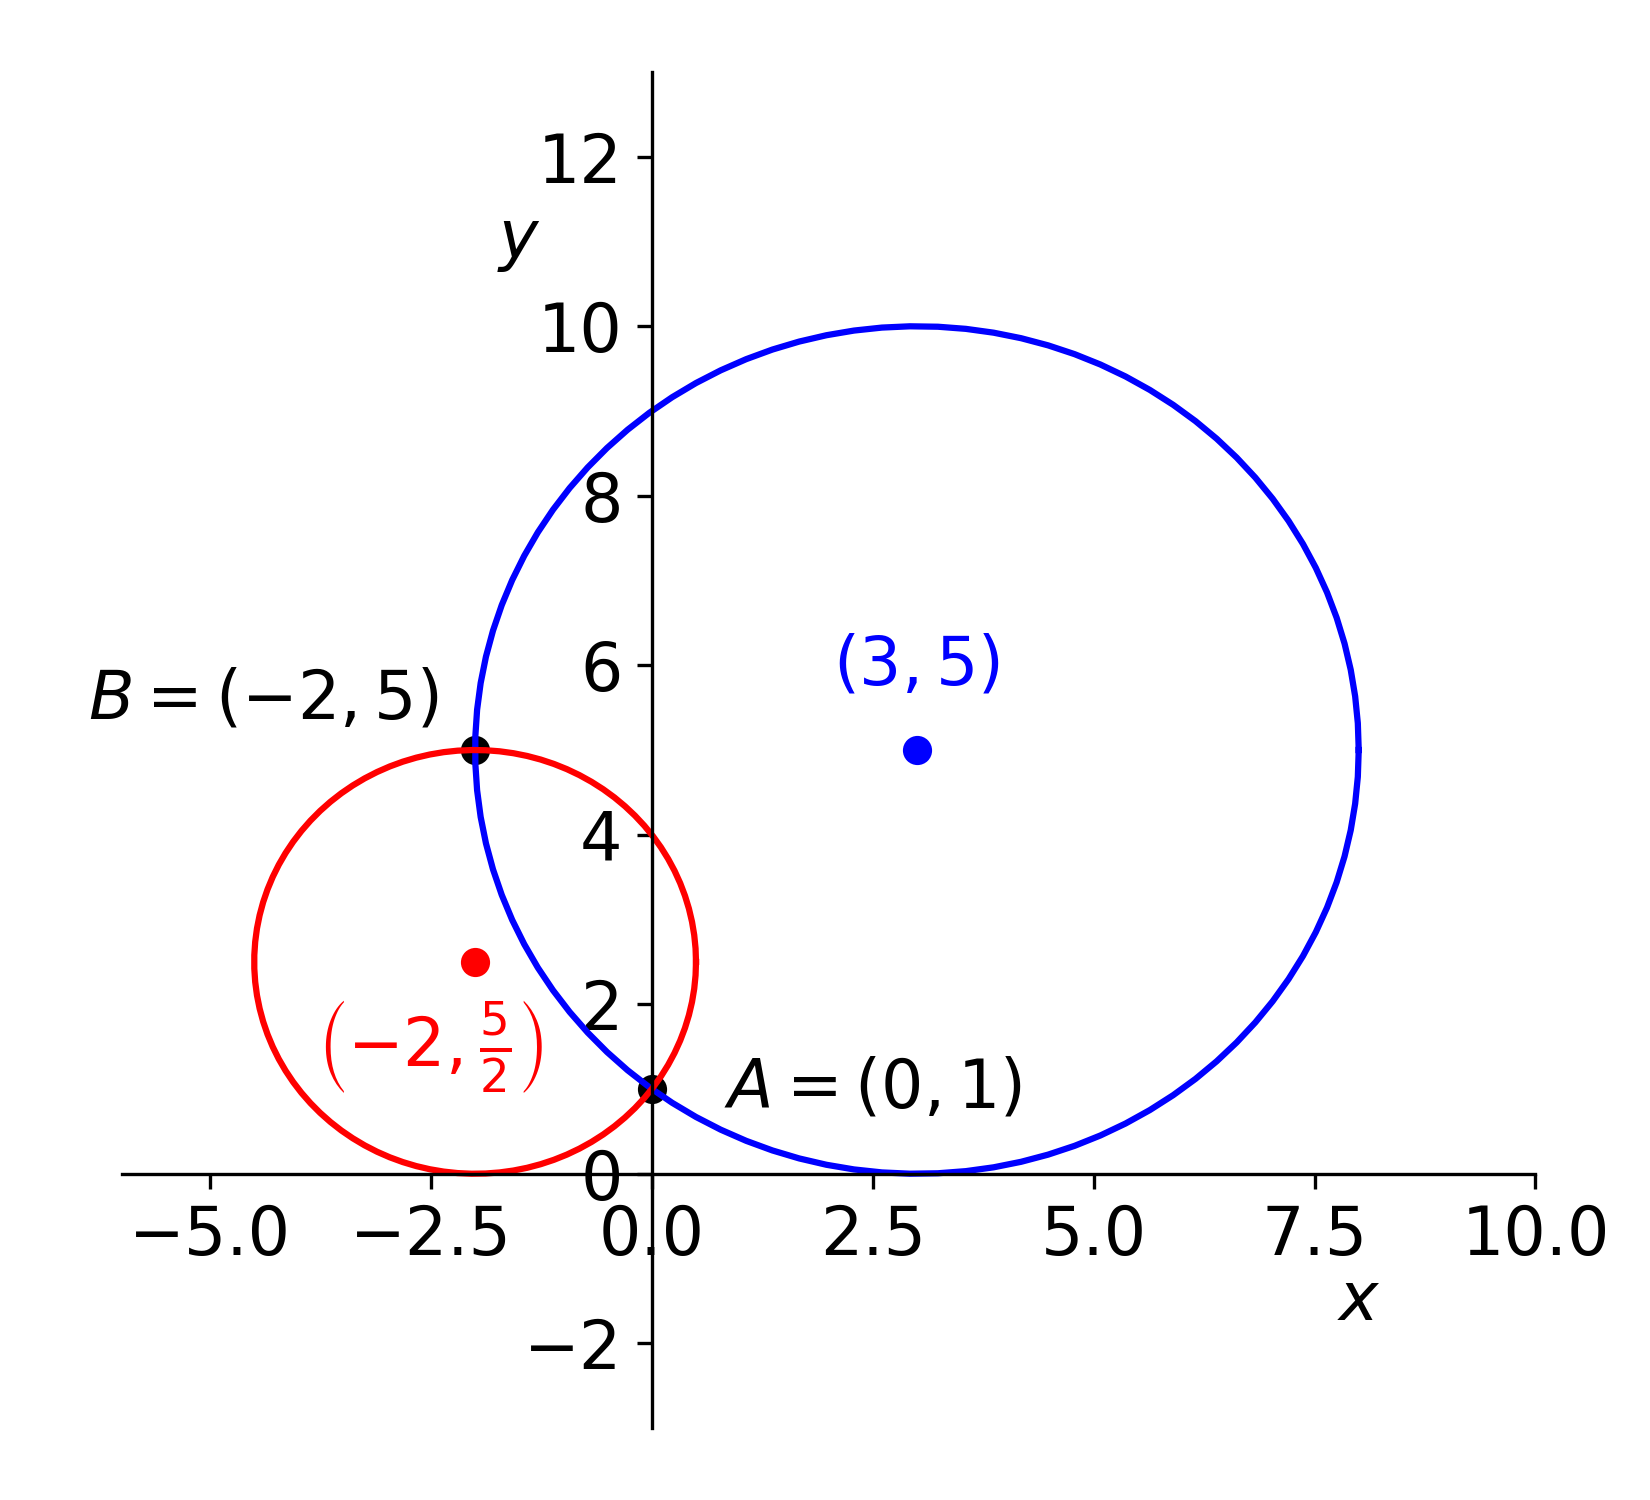
\includegraphics[width=0.5\textwidth, alt={Sketch of the two circles that cross at $A=(0,1)$ and $B=(-2,5)$ and touch the $x$-axis.}]{Figures/Section1/Ex_115.png}
    \end{center}
\fi

\end{solution}

\newtexpage
\subsection{Explicit, implicit and parametric relations}
\label{sec:relations}

\begin{learningoutcomes}
    \item Recognise when relations between variables are in explicit, implicit or parametric form
    \item Reformulate explicit equations into parametric and implicit forms.
\end{learningoutcomes}

\subsubsection{Implicit relations}

An explicit relation expresses the \textbf{dependent variable} (\textit{e.g.} $y$) as a function of the \textbf{independent variable } (\textit{e.g.} $x$), and so has the form $y=f(x)$. An example we have already met is the straight-line equation $
y=mx+c$.

\[
f(x,y)=d,
\]
for some constant $d$. For a given value of $x$, there may be multiple $y$ values that satisfy this (and vice versa). An example we have already met is the equation of a circle $(x-a)^2+(y-b)^2=R^2.$

In some cases, it is not possible to write a relation explicitly as $y=f(x)$. For example,
\[
4x+8y+\sin(\pi x)+\cos(\pi y)=1
\]
which is plotted in figure \ref{fig:implicit} behaves like an explicit function, with one value of $y$ for each $x$, however, we cannot reformulate it as an explicit function. 
\begin{figure}[h!]
\centering
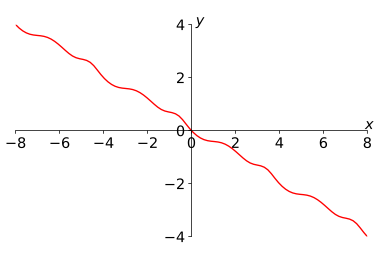
\includegraphics[width=0.5\textwidth]{Figures/Section1/121_implicit.png}
\caption{A plot of the implicit function $4x+8y+\sin(\pi x)+\cos(\pi y)=1$.}
\label{fig:implicit}
\end{figure}


\begin{example}[Video]
An ellipse can be written in implicit form as
\[
\frac{x^2}{100}+\frac{y^2}{25}=1.
\]
For $x=-10,-8,-6,0,6,8,10$, find the possible values of $y$ and hence draw the ellipse.
\end{example}

\begin{solution}
Rearrange to get $y$ in terms of $x$:
\[\blank{\frac{y^2}{25}=1-\frac{x^2}{100}}\]
\[
y=\blank{\pm5\sqrt{1-\frac{x^2}{100}}}=\blank{\pm\frac12\sqrt{100-x^2}}
\]
Substitution gives
\[
\begin{array}{c|rrrrrrr}
x&-10&-8&-6&0&6&8&10\\ \hline
y&\blank{0}&\blank{\pm3}&\blank{\pm4}&\blank{\pm5}&\blank{\pm4}&\blank{\pm3}&\blank{0}
\end{array}
\]
\begin{center}
\ifcsname insertBlanks\endcsname
    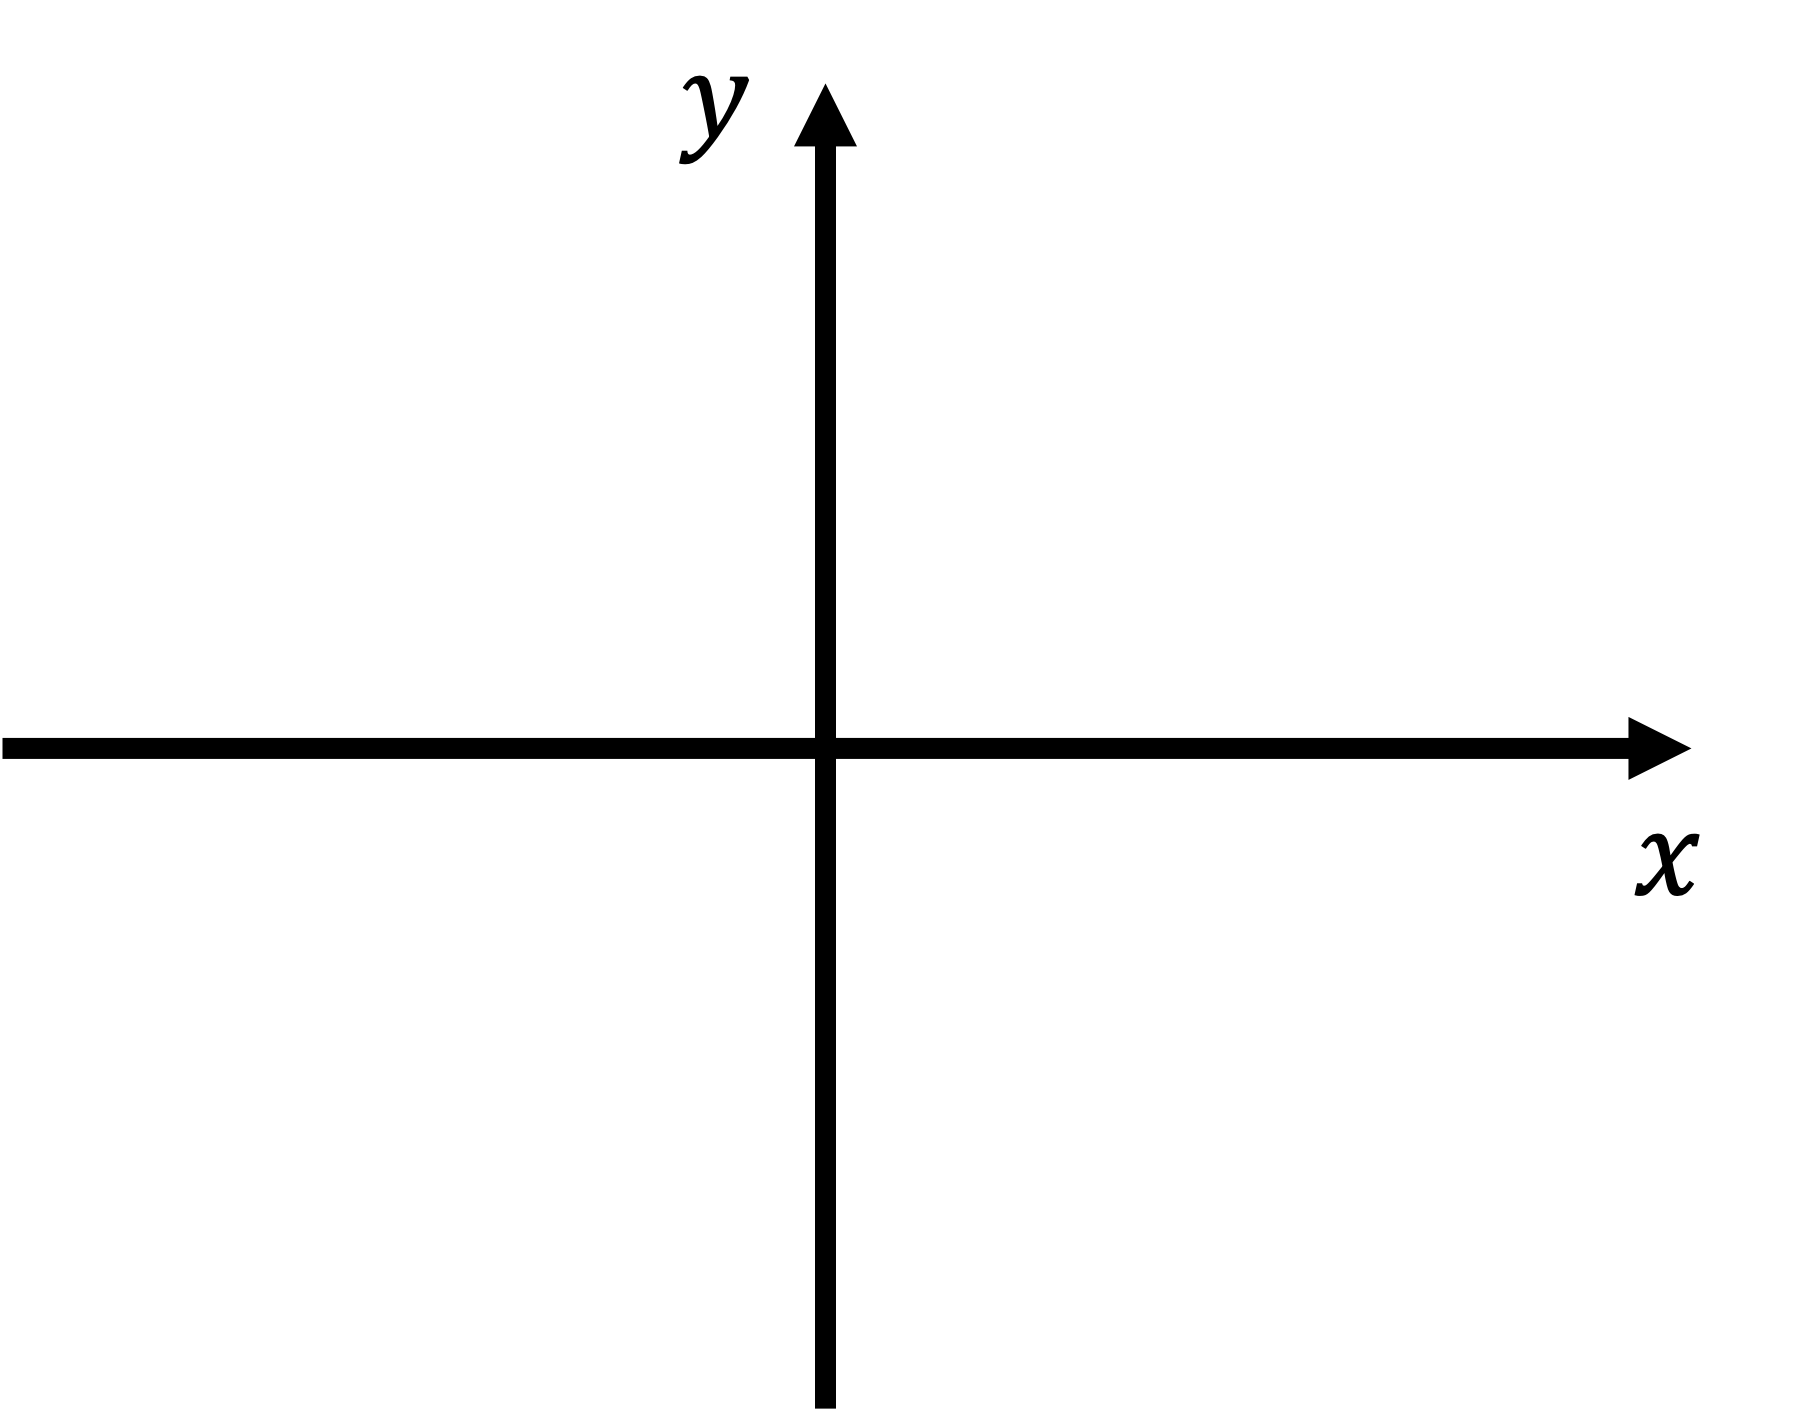
\includegraphics[width=0.5\textwidth]{Figures/Section1/example_121_frame.png}
\else
    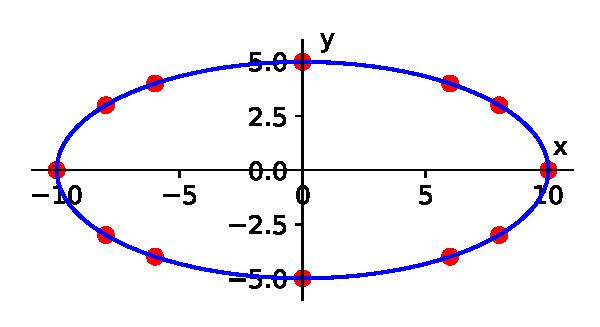
\includegraphics[width=0.5\textwidth]{Figures/Section1/example_121.pdf}
\fi
\end{center}
\end{solution}

\subsubsection{Parametric relations}

A \textbf{parametric relation} between $x$ and $y$ has the form
\[
x=f(t), \qquad y=g(t).
\]
So $x$ and $y$ are both functions of the parameter $t$. For example, the equation of a circle in parametric form is given by
\[
x=a+R\cos t, \qquad y=b+R\sin t,
\]
for $0\leq t<2\pi$. The interactive animation in figure \ref{anim:parametric} demonstrates how parametric relations can be visualised by making the parameter $t$ the coordinate of the third dimension. 

\begin{figure}
    \iflatexml
            \<div id="parametric-curve-widget" data-r="1">\</div> 
            \<script src="https://cdn.plot.ly/plotly-3.0.1.min.js">\</script>
            \<script src="bmluser/parametric\_curve\_widget.js">\</script>
        \caption{Interactive plot of the parametric curve $x=\cos t$, $y=\sin t$. The colour goes from white to red as $t$ increases.}
    \else
    \centering
    \subfig{0.33}{Figures/Section1/parametric_curve_widget_xt.png}{$x-t$ plane}
    \hfill
    \subfig{0.33}{Figures/Section1/parametric_curve_widget_yt.png}{$y-t$ plane}
    \hfill
    \subfig{0.25}{Figures/Section1/parametric_curve_widget_xy.png}{$x-y$ plane}
    \caption{Screenshots of the interactive plot of the parametric curve $x=\cos t$, $y=\sin t$, available in the html version of these notes. The colour goes from white to red as $t$ increases.}
    \fi
    \label{anim:parametric}
\end{figure}


\begin{example}[DIY]
Express the circle with centre at $(2,3)$ and radius 4 in parametric form.
\end{example}

\begin{blanksol}
In parametric form
\[
x=a+R\cos t,
\qquad
y=b+R\sin t.
\]
For $a=2$, $b=3$, and $R=4$, this gives
\[
x=2+4\cos t,
\qquad y=3+4\sin t,
\]
for $0\leq t<2\pi$.
\end{blanksol}

Given $x=f(t)$ and $y=g(t)$, it may or may not be possible to express $y$ directly as a function of $x$. For example, consider the parametric relation $x=t^2$, $y=t^4$. It can be written as $y=x^2$. However, for all values of $t$, $x$ can only be positive (see figure \ref{fig:parametric}).

\begin{figure}[h!]
\centering
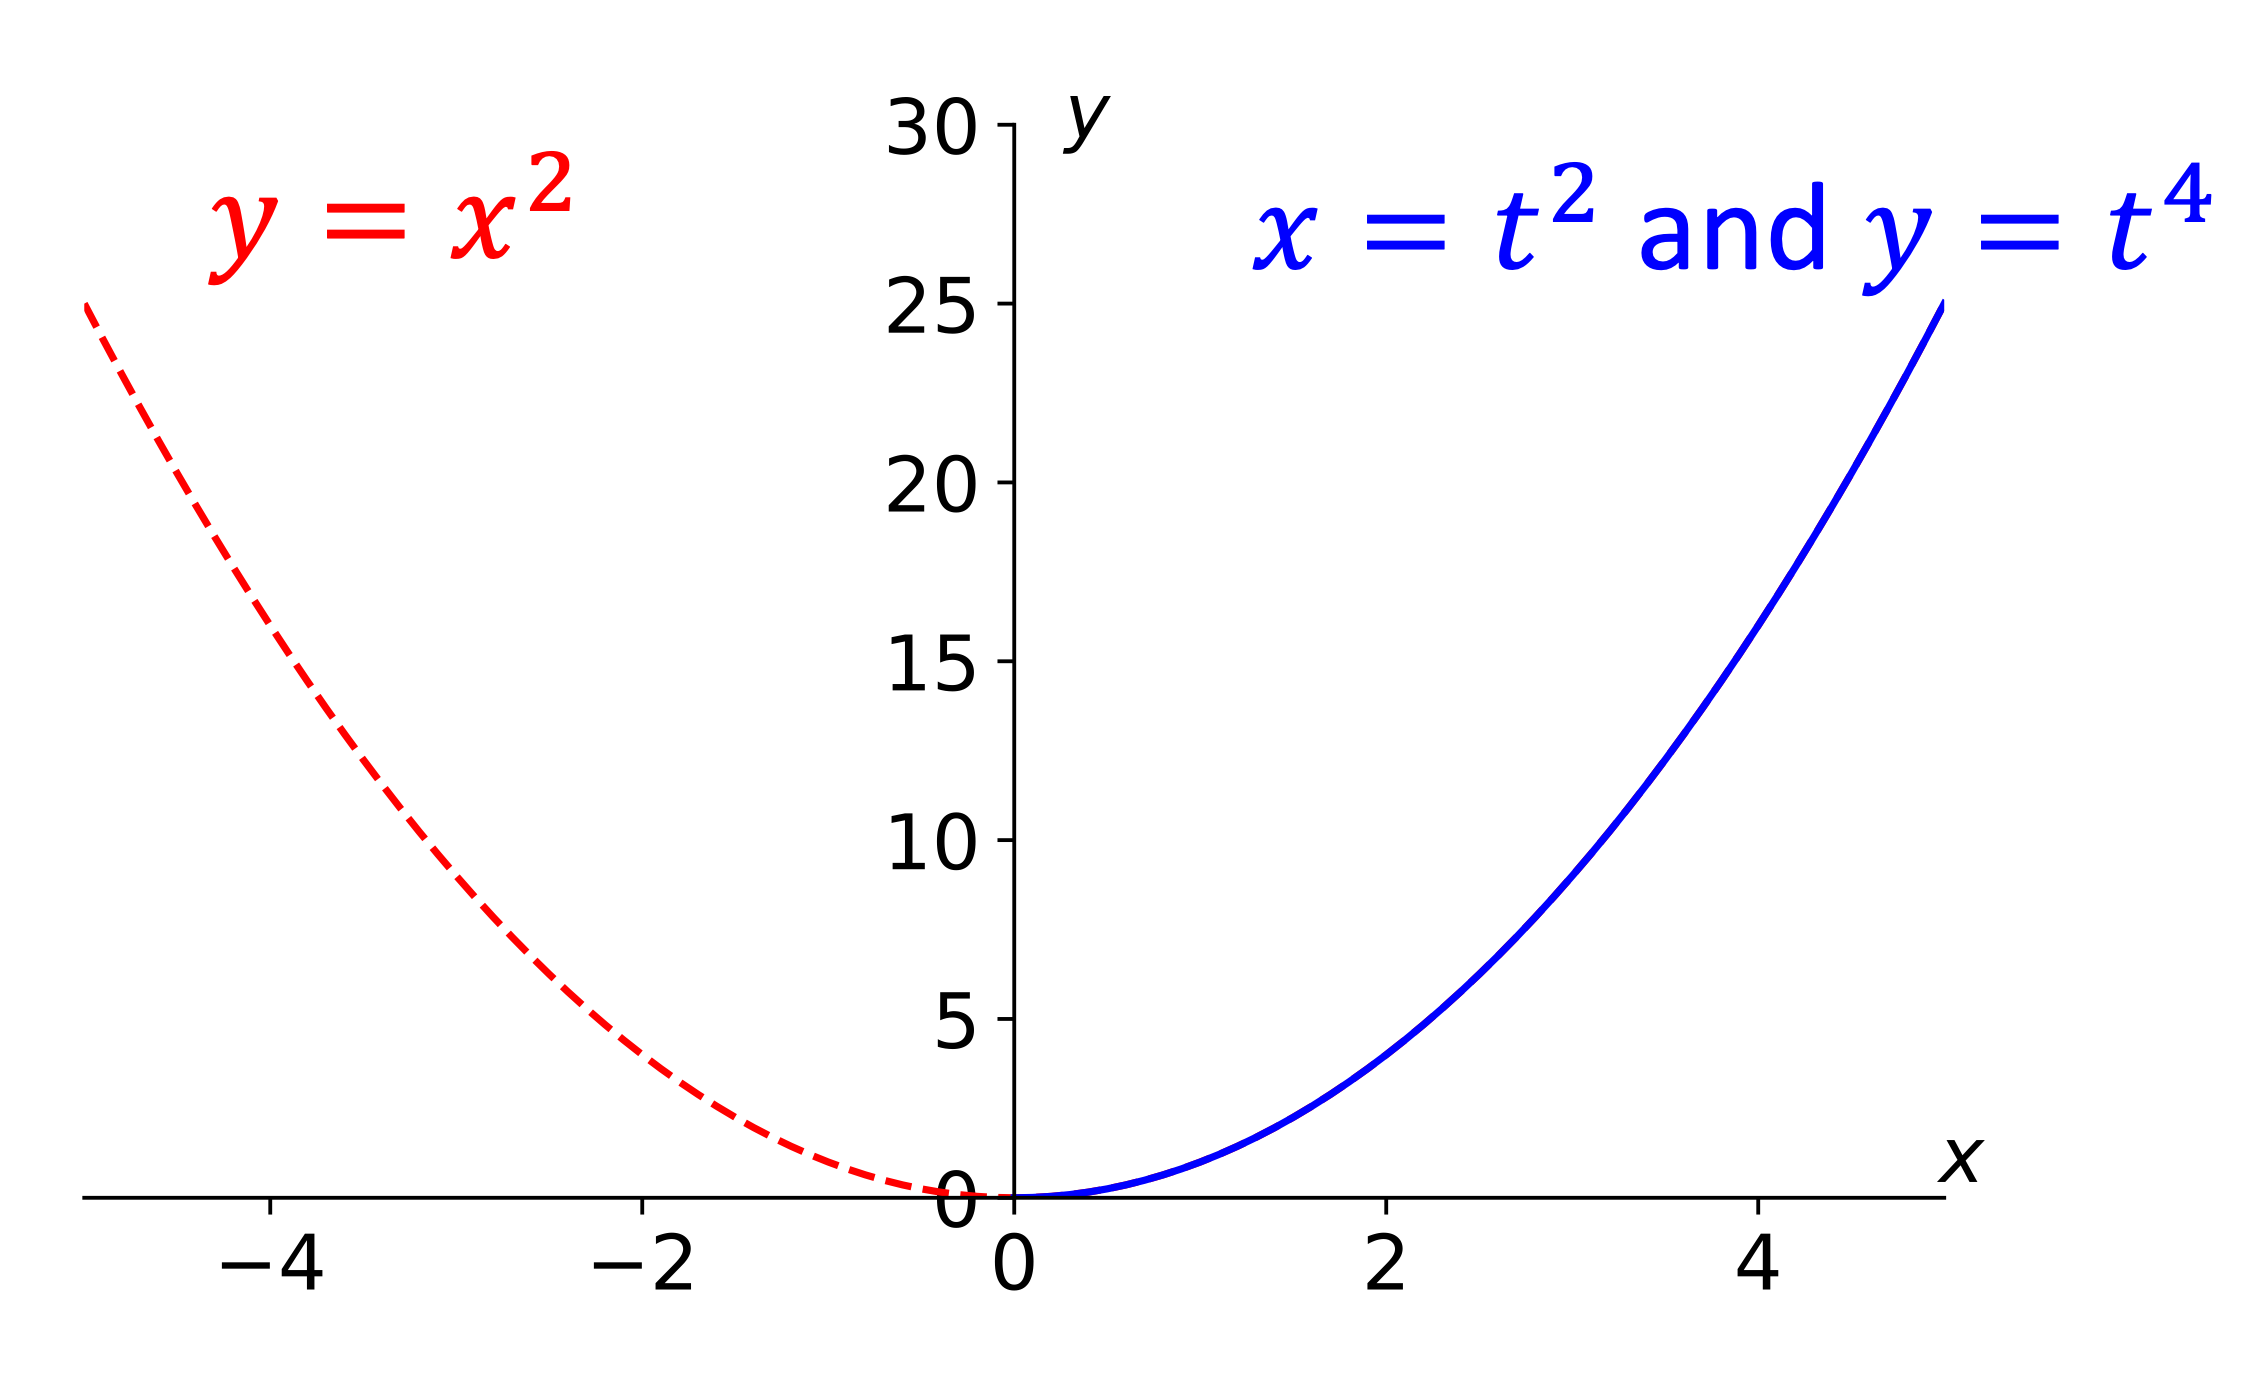
\includegraphics[width=0.5\textwidth]{Figures/Section1/122_parametric.png}
\caption{Comparison of the function $y=x^2$ and the parametric relation $x=t^2$, $y=t^4$.}
\label{fig:parametric}
\end{figure}

A general method to write parametric equations in explicit form is:
\begin{itemize}
\item rearrange the equation for the \textbf{independent variable} in terms of the parameter, i.e. rewrite $x=f(t)$ into $t=h(x)$;
\item substitute this into the equation for the \textbf{dependent variable}, i.e. replace $t$ with $h(x)$ in $y=g(t)$.
\end{itemize}

\begin{example}[Lecture]
Sodium oxide ($\mathrm{Na_2O}$) is placed in water producing sodium hydroxide:
\[
\mathrm{Na_2O+H_2O\longrightarrow 2NaOH}.
\]
The number of $\mathrm{Na_2O}$ and $\mathrm{NaOH}$ molecules in solution at time $t\geq0$ is given by
\[
x=x_0e^{-\alpha t} \qquad\text{and}\qquad y=2x_0\left(1-e^{-\alpha t}\right)
\]
respectively, where $x_0$ is the initial number of molecules of $\mathrm{Na_2O}$. Write $y$ as a function of $x$, noting any restrictions on their values.
\end{example}

\begin{solution}
Find substitution for $t$ in terms of $x$:
\[
\blank{e^{-\alpha t}=\frac{x}{x_0}}.
\]
Substitute into equation for $y$:
\[
\blank{y=2(x_0-x).}
\]
$x$ is a decreasing function of $t$, since $t\geq0$, the minimum and maximum $x$ values are
\[
\blank{0<x\leq x_0.}
\]
$y$ is an increasing function of $t$, the minimum and maximum $y$ values are
\[
\blank{0\leq y<2x_0.}
\]
\end{solution}

The straight line and the circle can both be expressed in parametric and implicit form.

\textbf{Straight Line}
\begin{itemize}
    \item Implicit: $ax+by=p$.
    \item Parametric: $x=bt$, $y=\frac{p}{b}-at$.
    \item Explicit: $y=-\frac{a}{b}x+\frac{p}{b}=mx+c$.
\end{itemize}

\textbf{Circle}
\begin{itemize}
\item Implicit: $(x-a)^2+(y-b)^2=R^2$.
\item Parametric: $x=a+R\cos t$, $y=b+R\sin t$.
\item Explicit: $y=b\pm\sqrt{R^2-(x-a)^2}$.
\end{itemize}

\subsection{Partial fractions}
\label{sec:partial_fracs}

\begin{learningoutcomes}
\item Simplify proper and improper compound fractions into partial fractions form
\end{learningoutcomes}

\subsubsection{Partial fractions in general}

What do we mean by ``partial fractions''? Consider the following sum of two fractions:
\[
\frac{1}{x+1}+\frac{3}{x-2}.
\]
We can put them over a common denominator to express as a single fraction (see figure \ref{fig:partial_frac}):
\[
\frac{4x+1}{(x+1)(x-2)}.
\]
Partial fraction decomposition is about \textbf{reversing} this operation. This is often useful for differentiation and integration.

\begin{figure}[h!]
    \centering
    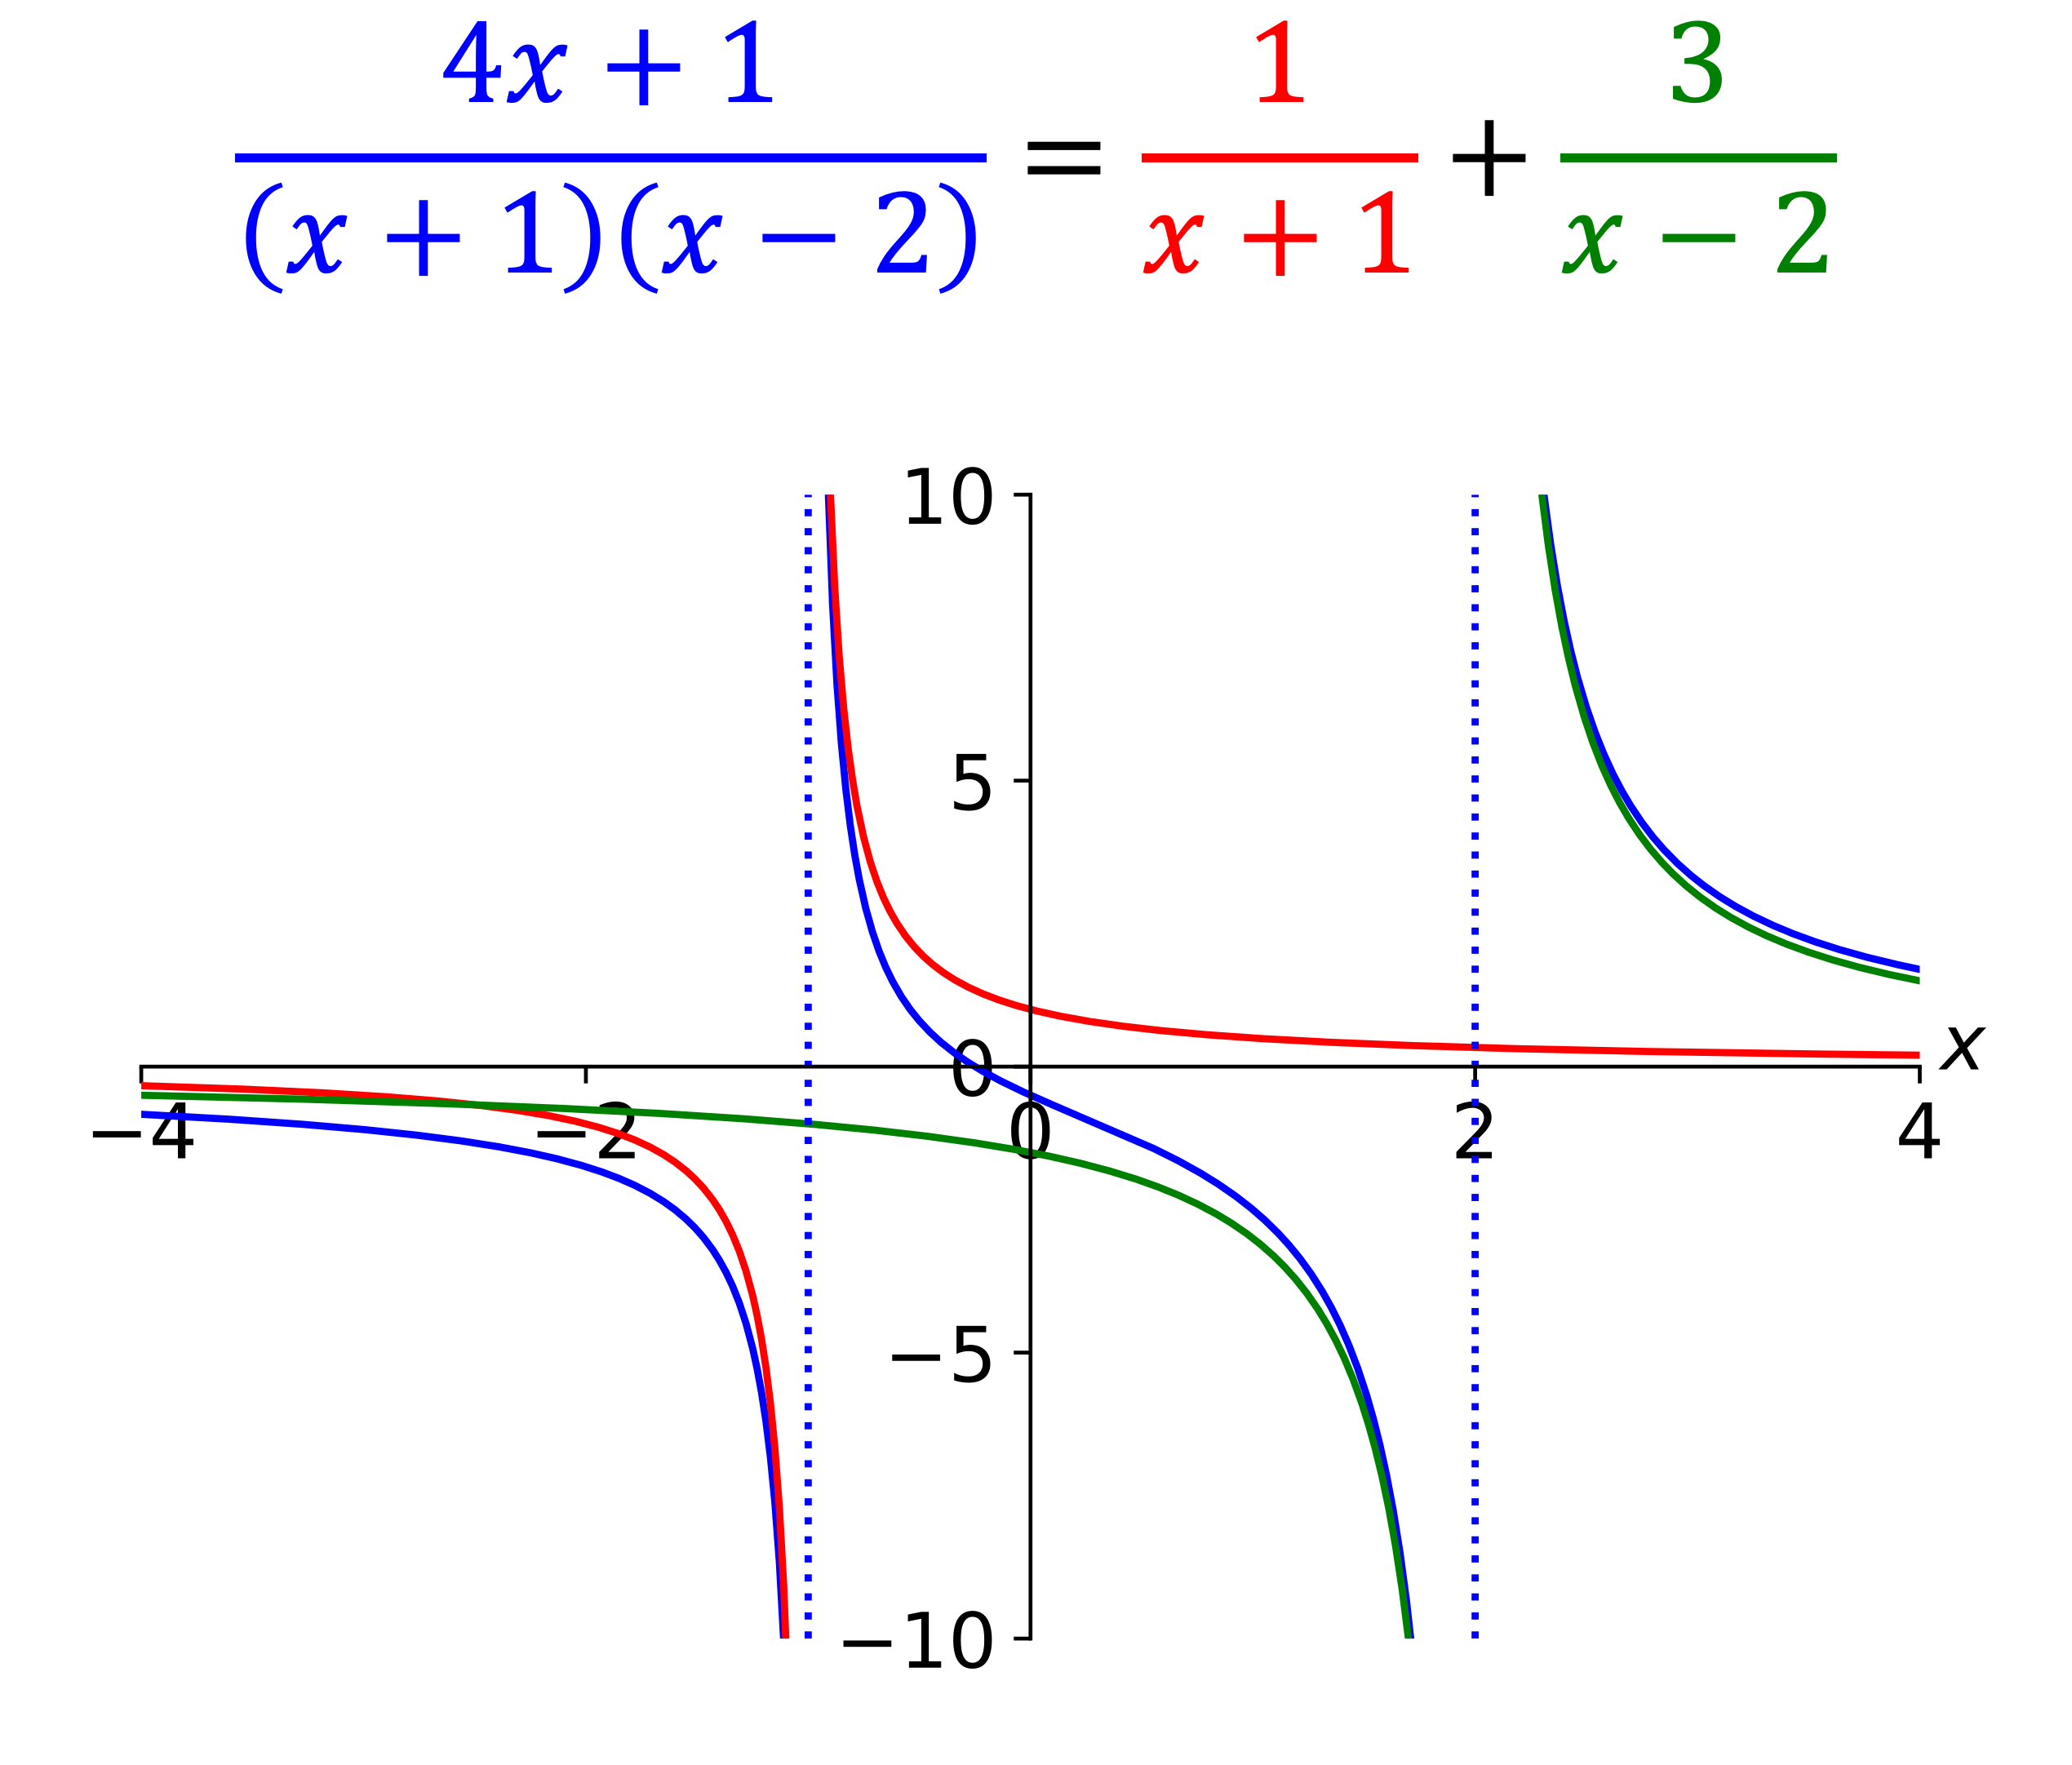
\includegraphics[width=0.5\textwidth]{Figures/Section1/131_partial_frac.png}
    \caption{Plots of the irreducible fractions $\frac{1}{x+1}$ + and $\frac{3}{x-2}$ and their sum, equivalent to $\frac{4x+1}{(x+1)(x-2)}$.}
    \label{fig:partial_frac}
\end{figure}

\begin{definitions}
    \begin{itemize}
    \item A \textbf{rational fraction} has a numerator and denominator that are both polynomials.
    \item The \textbf{degree} of a polynomial is the largest power in the polynomial, \textit{e.g.} $x^3+x^2-x+1=0$ is degree 3.
    \item Defining $d$ as the degree of the denominator and $n$ as the degree of the numerator, then a \textbf{proper fraction} is a rational fraction where $d>n$. An \textbf{improper fraction} is a rational fraction where $d\leq n$.
    \end{itemize}
\end{definitions}

\subsubsection{Partial fractions for proper fractions}

\textbf{Case 1: Linear function divided by factorising quadratic.} A linear function divided by a factorising quadratic can be written in the form
\[
\frac{\text{linear}}{(x-a)(x-b)}=\frac{A}{x-a}+\frac{B}{x-b}.
\]
To find $A$ and $B$, first multiply both sides by the denominator $(x-a)(x-b)$ to yield
\[
\text{linear}=A(x-b)+B(x-a).
\]
This equation must hold \textbf{for all} $x$. So, set $x=a$ to find $A$ (in terms of $a$, $b$, and the linear function) and set $x=b$ to find $B$ (in terms of $a$, $b$, and the linear function).

\begin{example}[Lecture]
Express in partial fractions form
\[
\frac{x-4}{2x^2+5x-3}.
\]
\end{example}

\begin{solution}
Factorise the denominator
\[
2x^2+5x-3=\blank{(x+3)(2x-1)}.
\]
Write the form of the solution
\[
\frac{x-4}{(x+3)(2x-1)}=\blank{\frac{A}{x+3}+\frac{B}{2x-1}}.
\]
Multiply through by the denominator
\[
x-4=\blank{A(2x-1)+B(x+3)}.
\]
Solve for $A$ and $B$\par
\blankpar{ Substituting $x=-3$ gives $-7=-7A$, therefore $A=1$}\par
\blankpar{ Substituting $x=1/2$ gives $-7/2=-7B/2$, therefore $B=-1$}\par
and so
\[
\frac{x-4}{2x^2+5x-3}=\blank{\frac{1}{x+3}-\frac{1}{2x-1}}.
\]
\end{solution}

\textbf{Case 2: Quadratic function divided by a factorising cubic.} A quadratic function divided by a factorising cubic can be written in the form
\[
\frac{\text{quadratic}}{(x-a)(x-b)(x-c)}=\frac{A}{x-a}+\frac{B}{x-b}+\frac{C}{x-c}.
\]
To find $A$, $B$ and $C$, multiply through by the denominator:
\[
\text{quadratic}=A(x-b)(x-c)+B(x-a)(x-c)+C(x-a)(x-b).
\]
Then set $x=a$ to find $A$, $x=b$ to find $B$, and $x=c$ to find $C$.

Case 1 and 2 generalise to any proper fraction with linear factors on the denominator:
\[
\frac{\text{degree }n-1\text{ polynomial}}{(x-x_1)(x-x_2)\cdots(x-x_n)}
=
\frac{A_1}{x-x_1}+\frac{A_2}{x-x_2}+\cdots+\frac{A_n}{x-x_n}.
\]

\begin{example}[Video]
Express in partial fractions form
\[
\frac{2x^2+8x+18}{x(x+2)(x-3)}.
\]
\end{example}

\begin{solution}
The denominator contains 3 linear factors, so the correct form is
\[
\frac{2x^2+8x+18}{x(x+2)(x-3)}=\blank{\frac{A}{x}+\frac{B}{x+2}+\frac{C}{x-3}}.
\]
Multiplying both sides by the denominator:
\[
\blank{2x^2+8x+18=A(x+2)(x-3)+Bx(x-3)+Cx(x+2)}.
\]
3) This must hold for all $x$, so substitute $x=0$ to cancel $B$ and $C$ terms:
\[
\blank{18=A(2)(-3)=-6A \qquad \therefore \; A=-3.}
\]
Substitute $x=-2$ to cancel $A$ and $C$ terms:
\[
\blank{8-16+18=B(-2)(-5) \qquad \therefore \; -10B=10 \qquad \therefore \; B=1.}
\]
Substitute $x=3$ to cancel $A$ and $B$ terms:
\[
\blank{18+24+18=C(3)(5) \qquad \therefore \; 15C=60 \qquad \therefore \; C=4.}
\]
And so
\[
\frac{2x^2+8x+18}{x(x+2)(x-3)}=\blank{-\frac{3}{x}+\frac{1}{x+2}+\frac{4}{x-3}.}
\]
\end{solution}

\textbf{Case 3: Repeated factor in the denominator.} A repeated factor in the denominator results in two fractions, one with a square on the denominator, e.g.
\[
\frac{\text{quadratic}}{(x-a)^2(x-b)}=\frac{A}{x-a}+\frac{B}{(x-a)^2}+\frac{C}{x-b}.
\]
Multiplying both sides by the denominator:
\[
\text{quadratic}=A(x-a)(x-b)+B(x-b)+C(x-a)^2.
\]
Setting $x=a$ and $x=b$ only gives two of $A$, $B$, $C$. It is necessary to find the third by comparing coefficients of a power of $x$ (e.g. comparing constants by setting $x=0$).

This case also generalises to factors repeated $n$ times, e.g.
\[
\frac{\text{degree }n\text{ polynomial}}{(x-a)(x-b)^n}=\frac{A}{x-a}+\frac{B_1}{x-b}+\cdots+\frac{B_n}{(x-b)^n}.
\]

\begin{example}[DIY]
Write down the partial fractions form for
\[
\frac{x+9}{x(x^2-6x+9)},
\]
but \textbf{do not} find the values of the coefficients.
\end{example}

\begin{blanksol}
Factorise the denominator:
\[
x^2-6x+9=(x-3)^2.
\]
Three terms required for $x$, $x-3$, and $(x-3)^2$. Therefore, the partial fraction form is
\[
\frac{x+9}{x(x^2-6x+9)}=\frac{A}{x}+\frac{B}{x-3}+\frac{C}{(x-3)^2}.
\]
\end{blanksol}

\textbf{Case 4: Irreducible quadratic in the denominator.} An irreducible quadratic factor in the denominator results in a term of the form $\frac{Ax+B}{\text{quadratic}}$, \textit{e.g.}
\[
\frac{\text{quadratic}}{(x^2+2x+9)(x-1)}=\frac{Ax+B}{x^2+2x+9}+\frac{C}{x-1}.
\]
Once again, it is necessary to use comparison of coefficients in order to find some of the values $A$, $B$, $C$ etc.

This rule generalises to irreducible polynomials of degree $n$, e.g.
\[
\frac{\text{degree }n\text{ polynomial}}{(x-a)(\text{irreducible degree }n\text{ polynomial})}
=
\frac{A}{x-a}+\frac{B_{n-1}x^{n-1}+\cdots+B_1x+B_0}{\text{irreducible degree }n\text{ polynomial}}.
\]

\begin{example}[Video]
Express in partial fractions form
\[
\frac{x^2}{(x-1)(x^2+3x-3)}.
\]
\end{example}

\begin{solution}
The denominator cannot be factorised further, so the correct form is
\[
\frac{x^2}{(x-1)(x^2+3x-3)}=\blank{\frac{A}{x-1}+\frac{Bx+C}{x^2+3x-3}.}
\]
Multiplying both sides by the denominator and collect powers of $x$:
\begin{align}
    \blank{x^2} &= \blank{A(x^2+3x-3) + (Bx+C)(x-1)} \\
    \blank{x^2} &= \blank{(A+B)x^2+(3A-B+C)x-3A-C} \, .
\end{align}
Compare coefficients of powers of $x$:
\[
x^0:\quad \blank{0=-3A-C \qquad \therefore C=-3A,}
\]
\[
x:\quad \blank{0=3A-B+C \qquad \therefore B=0,}
\]
\[
x^2:\quad \blank{1=A+B \qquad A=1 \qquad \therefore C=-3.}
\]
And so
\[
\frac{x^2}{(x-1)(x^2+3x-3)}=\blank{\frac{1}{x-1}-\frac{3}{x^2+3x-3}.}
\]
\end{solution}

\subsubsection{Partial fractions for improper fractions}

If a rational function has a denominator of degree $n$ and a numerator of degree $n+m$, then the resultant partial fraction will include a polynomial of degree $m$. To find the coefficients, multiply both sides by the denominator and either substitute meaningful values of $x$ or compare coefficients of powers of $x$.

\begin{example}[Lecture]
Find the partial fractions form of
\[
\frac{3(x+1)^2}{x^2+x-2}.
\]
\end{example}

\begin{solution}
Factorise the denominator:
\[
\blank{x^2+x-2=(x-1)(x+2).}
\]
Identify correct form:
\[
\blank{\frac{3(x+1)^2}{(x-1)(x+2)}=A+\frac{B}{x-1}+\frac{C}{x+2}.}
\]
Multiply through and solve for coefficients:
\[
\frac{3(x+1)^2}{x^2+x-2}=\blank{3+\frac{4}{x-1}-\frac{1}{x+2}.}
\]
\end{solution}

\begin{example}[Video]
Find the partial fractions form for
\[
\frac{5x^6-50x^5+386x^4-1074x^3+644x^2+1174x-1354}{(x-2)^2(x^2-6x+50)},
\]
but \textbf{do not} find the values of the coefficients.
\end{example}

\begin{solution}
Check the degree of the numerator ($n$) and denominator ($d$):
\[
n=\blank{6} \qquad\text{and}\qquad d=\blank{4} \qquad\text{and so}\qquad \blank{n-d=2.}
\]
Therefore the partial fractions form contains a quadratic.

Check if the denominator factorises further \par
\blankpar{It does not.}

Write the terms for the repeated root and the quadratic:
\[
\blank{Ax^2+Bx+C+\frac{D}{x-2}+\frac{E}{(x-2)^2}+\frac{Fx+G}{x^2-6x+50}.}
\]
\end{solution}
